\documentclass[12pt, a4paper]{article}

% ── Codificación y lengua ─────────────────────────────────────────────────────
\usepackage[utf8]{inputenc}
\usepackage[T1]{fontenc}
\usepackage[spanish]{babel}

% ── Tipografía y diseño ───────────────────────────────────────────────────────
\usepackage{lmodern}
\usepackage{microtype}
\usepackage{geometry}
\geometry{
  a4paper,
  top=2.5cm, bottom=2.5cm,
  left=3cm,  right=2.5cm
}
\usepackage{setspace}
\onehalfspacing

% ── Sangría en todos los párrafos (incluido el primero de cada sección) ───────
\usepackage{indentfirst}
\setlength{\parindent}{1.5em}
\setlength{\parskip}{4pt}

% ── Colores (solo para elementos decorativos, no para texto) ──────────────────
\usepackage[dvipsnames]{xcolor}
\definecolor{azuloscuro}{RGB}{31, 56, 100}
\definecolor{azulmedio}{RGB}{46, 117, 182}
\definecolor{grisclaro}{RGB}{245, 245, 245}
\definecolor{amarillotodo}{RGB}{255, 243, 205}

% ── Encabezados y secciones (texto en negro) ──────────────────────────────────
\usepackage{titlesec}
\titleformat{\section}
  {\large\bfseries}{{\thesection.}}{0.6em}{}
  [\vspace{-4pt}\color{azulmedio}\rule{\linewidth}{1pt}\vspace{2pt}]
\titleformat{\subsection}
  {\normalsize\bfseries}{{\thesubsection.}}{0.5em}{}
\titleformat{\subsubsection}
  {\normalsize\itshape}{{\thesubsubsection.}}{0.5em}{}
\titlespacing{\section}{0pt}{18pt}{8pt}
\titlespacing{\subsection}{0pt}{12pt}{4pt}

% ── Encabezado y pie de página ────────────────────────────────────────────────
\usepackage{fancyhdr}
\pagestyle{fancy}
\fancyhf{}
\fancyhead[L]{\small\textit{Clasificación Automática de Retinopatía Diabética}}
\fancyhead[R]{\small\textit{PIM --- Curso 2025/2026}}
\fancyfoot[C]{\small\thepage}
\renewcommand{\headrulewidth}{0.4pt}
\renewcommand{\footrulewidth}{0pt}
\setlength{\headheight}{14.5pt}

% ── Tablas ────────────────────────────────────────────────────────────────────
\usepackage{booktabs}
\usepackage{array}
\usepackage{tabularx}
\usepackage{multirow}
\usepackage{colortbl}

% ── Figuras ───────────────────────────────────────────────────────────────────
\usepackage{graphicx}
\usepackage{float}
\usepackage{caption}
\captionsetup{
  font=small,
  labelfont=bf,
  labelsep=period
}

% ── Matemáticas ───────────────────────────────────────────────────────────────
\usepackage{amsmath}
\usepackage{amssymb}

% ── Listas ────────────────────────────────────────────────────────────────────
\usepackage{enumitem}
\setlist[itemize]{itemsep=2pt, topsep=4pt}
\setlist[enumerate]{itemsep=2pt, topsep=4pt}

% ── Hipervínculos y referencias ───────────────────────────────────────────────
\usepackage[
  colorlinks=true,
  linkcolor=black,
  citecolor=black,
  urlcolor=black,
  pdftitle={Clasificación Automática de Retinopatía Diabética},
  pdfauthor={García Fernández, Véliz Ayala, Solano Martínez},
]{hyperref}
\usepackage[style=ieee, sorting=none]{biblatex}
\addbibresource{referencias.bib}

% ── Otros ─────────────────────────────────────────────────────────────────────
\usepackage{tocbibind}
\usepackage{xspace}

% ── Comandos propios ──────────────────────────────────────────────────────────
\newcommand{\kappados}{$\kappa^2$\xspace}

% Caja amarilla para marcar contenido pendiente (texto en negro)
\newcommand{\pendiente}[1]{%
  \vspace{4pt}%
  \colorbox{amarillotodo}{%
    \parbox{\dimexpr\linewidth-2\fboxsep}{%
      \small\itshape%
      $\blacktriangleright$ \textbf{[PENDIENTE]:} #1%
    }%
  }%
  \vspace{4pt}%
}

% Caja resaltada para "Problema" y "Solución" en cada experimento.
% Implementada como tabularx con color de fondo para garantizar que respeta
% los márgenes del texto (evita overfull hbox).
\definecolor{cajagris}{RGB}{248, 246, 240}
\definecolor{bordegris}{RGB}{211, 209, 199}
\newcommand{\experimentobox}[2]{%
  \vspace{3pt}%
  \noindent%
  \begin{tabularx}{\linewidth}{|>{\columncolor{cajagris}}X|}
    \hline
    \small\textbf{#1}\ #2 \\
    \hline
  \end{tabularx}%
  \vspace{3pt}%
}

% ══════════════════════════════════════════════════════════════════════════════
\begin{document}
\pagenumbering{gobble}

% ══════════════════════════════════════════════════════════════════════════════
%  PORTADA
% ══════════════════════════════════════════════════════════════════════════════
\begin{titlepage}
  \centering

  \begin{minipage}{\textwidth}
    \color{azuloscuro}\rule{\textwidth}{4pt}
  \end{minipage}

  \vspace{2.5cm}

  {\Huge\bfseries
    Clasificación Automática de\\[6pt]
    Retinopatía Diabética
  }

  \vspace{0.5cm}
  {\large\itshape
    Pipeline Completo de Clasificación por Gradación de Severidad
  }

  \vspace{0.4cm}
  \color{azulmedio}\rule{0.6\textwidth}{1.5pt}\color{black}

  \vspace{2cm}

  \begin{tabular}{rl}
    \textbf{Asignatura:}       & Procesamiento de Imagen en Medicina \\[4pt]
    \textbf{Curso académico:}  & 2025 -- 2026 \\[4pt]
    \textbf{Fecha de entrega:} & 24 de abril de 2026 \\
  \end{tabular}

  \vspace{2cm}

  {\large\bfseries Integrantes del grupo}\\[0.6cm]
  \begin{tabular}{c}
    Javier García Fernández    \\[4pt]
    Miguel Ángel Véliz Ayala  \\[4pt]
    Martín Solano Martínez     \\
  \end{tabular}

  \vfill

  \begin{minipage}{\textwidth}
    \color{azuloscuro}\rule{\textwidth}{4pt}
  \end{minipage}

\end{titlepage}

% ══════════════════════════════════════════════════════════════════════════════
%  RESUMEN
% ══════════════════════════════════════════════════════════════════════════════
\newpage
\pagenumbering{roman}

\phantomsection
\section*{Resumen}
\addcontentsline{toc}{section}{Resumen}

Este trabajo aborda la clasificación automática de la retinopatía diabética (RD) en
cinco grados de severidad clínica, desde grado~0 (sin RD) hasta grado~4
(proliferativa), a partir del dataset público APTOS~2019. Se construye un pipeline
completo basado en EfficientNetBN-B3 (MONAI) con preprocesamiento específico para
retinografías mediante máscara circular y CLAHE, y se diseñan y comparan diez
experimentos que abordan las principales limitaciones del modelo base: desbalance de
clases~(Exp.~A), radiómica cuantitativa con PyRadiomics~(Exp.~B), clasificación
zero-shot con BiomedCLIP~(Exp.~C), pipelines jerárquicos~(Exp.~D y E), regresión
ordinal a 384~px con optimización de umbrales~(Exp.~F), corrección de
\textit{shortcut learning} mediante preprocesado Ben~Graham~(Exp.~G), fusión
multimodal CNN\,+\,radiómica con LightGBM~(Exp.~I) y preentrenamiento en
APTOS~2015~(Exp.~J). La métrica principal es el kappa cuadrático ponderado~($\kappa^2$),
estándar en la literatura de gradación automática de RD. 

Los resultados demuestran que el preentrenamiento masivo en APTOS~2015 (Exp.~J) alcanza 
el máximo rendimiento global con un $\kappa^2$ de 0.8849, estableciendo un modelo 
altamente robusto ante la variabilidad de las imágenes. Por otro lado, la estrategia 
jerárquica en etapas (Exp.~D) destaca como la solución más eficaz para mejorar la 
precisión diagnóstica individual, logrando el F1-score más alto (0.63) y optimizando 
significativamente la detección de las clases críticas (G4). Cabe destacar que, aunque 
ciertos experimentos no supusieron saltos cuantitativos drásticos en el kappa global, 
su valor reside en una optimización estratégica que refuerza la consistencia diagnóstica 
y la fiabilidad en la detección de los estadios más graves de la enfermedad.

% ══════════════════════════════════════════════════════════════════════════════
%  ÍNDICE
% ══════════════════════════════════════════════════════════════════════════════
\newpage
\phantomsection
\tableofcontents

% ══════════════════════════════════════════════════════════════════════════════
%  CUERPO DEL DOCUMENTO
% ══════════════════════════════════════════════════════════════════════════════
\newpage
\pagenumbering{arabic}

% ══════════════════════════════════════════════════════════════════════════════
%  1. INTRODUCCIÓN
% ══════════════════════════════════════════════════════════════════════════════
\section{Introducción}

La \textbf{retinopatía diabética} (RD) es una complicación microvascular de la
diabetes mellitus y una de las principales causas de ceguera prevenible en el mundo.
Con más de 540 millones de adultos diabéticos estimados en 2023 y una prevalencia
de afectación retiniana en torno al 35\,\% de los pacientes~\cite{idf2023,who2023},
el cribado masivo mediante retinografías de fondo de ojo es una necesidad clínica
de primer orden. Sin embargo, la revisión manual de miles de imágenes por
oftalmólogos resulta inviable a gran escala, lo que motiva el desarrollo de sistemas
automáticos de gradación. Además, estos sistemas no solo permiten escalar el
cribado, sino que también facilitan y agilizan el trabajo del personal sanitario,
sirviendo como herramienta de apoyo en la clasificación de la enfermedad y en la
toma de decisiones clínicas. En este contexto, se emplea el dataset público APTOS~2019,
ampliamente utilizado en la literatura, que contiene retinografías etiquetadas según
el grado de severidad de la enfermedad, lo que permite evaluar de forma objetiva el
rendimiento de los modelos propuestos.

La enfermedad progresa en cinco estadios (Tabla~\ref{tab:grados}): desde la ausencia
de lesiones (G0) hasta la neovascularización proliferativa con riesgo de ceguera súbita
(G4), pasando por microaneurismas aislados (G1), hemorragias y exudados duros (G2) y
afectación vascular extensa en los cuatro cuadrantes (G3). Esta naturaleza ordinal del
problema, junto con el severo desbalance de clases del dataset ---G0 representa
$\sim$49\,\% del entrenamiento frente al $\sim$5\,\% de G3---, la ambigüedad entre
grados adyacentes, la pérdida de detalles finos al comprimir las imágenes a baja
resolución y el riesgo de \textit{shortcut learning} sobre artefactos de adquisición,
conforman los desafíos técnicos que este proyecto aborda de forma sistemática.

\begin{table}[H]
  \centering
  \caption{Escala de severidad de la retinopatía diabética.}
  \label{tab:grados}
  \begin{tabularx}{0.9\textwidth}{c l X}
    \toprule
    \rowcolor{azuloscuro!15}
    \textbf{Grado} & \textbf{Nombre} & \textbf{Características clínicas} \\
    \midrule
    0 & Sin RD        & Fondo de ojo normal. Sin lesiones visibles. \\
    \rowcolor{grisclaro}
    1 & Leve          & Microaneurismas aislados. \\
    2 & Moderada      & Hemorragias, exudados duros y anomalías vasculares. \\
    \rowcolor{grisclaro}
    3 & Severa        & Múltiples hemorragias, \textit{venous beading} e IRMA
                        en los cuatro cuadrantes. \\
    4 & Proliferativa & Neovascularización con riesgo de hemorragia vítrea
                        y desprendimiento de retina. \\
    \bottomrule
  \end{tabularx}
\end{table}

\newpage

El objetivo del proyecto es construir un pipeline reproducible y clínicamente
interpretable que parta de un baseline sólido (EfficientNetBN-B3, APTOS~2019,
224~px) y lo mejore de forma justificada mediante diez experimentos que atacan
cada una de las debilidades identificadas. Para ello, se emplea el dataset público
APTOS~2019, compuesto por retinografías etiquetadas en cinco grados de severidad,
lo que permite abordar el problema en un entorno realista y con datos clínicamente
relevantes. La métrica principal es el
\textbf{kappa cuadrático ponderado}~($\kappa^2$), que penaliza los errores
proporcionalmente al cuadrado de la distancia ordinal entre grados, alineándose
con la relevancia clínica de cada tipo de error. La elección de la RD como
problema de estudio responde, además, a la disponibilidad de datos públicos de
calidad (licencia CC~BY~4.0) y a que su naturaleza permite aplicar directamente
las técnicas del curso: preprocesamiento de imagen médica, aprendizaje profundo
con MONAI, radiómica cuantitativa e interpretabilidad con Grad-CAM.

\begin{figure}[H]
  \centering
  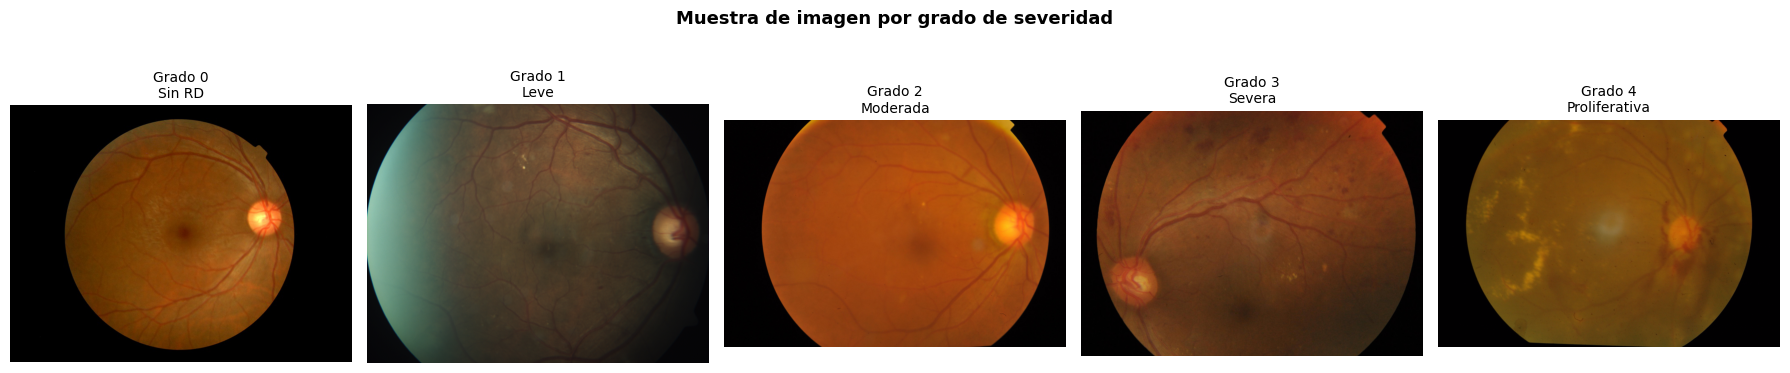
\includegraphics[width=\textwidth]{figura1.png}
  \caption{Retinografías representativas por grado de severidad (G0--G4).
    Las diferencias entre grados adyacentes son sutiles, lo que dificulta
    la gradación manual a gran escala.}
  \label{fig:grados}
\end{figure}

El resto del documento se organiza del siguiente modo: la Sección~\ref{sec:arte}
revisa el estado del arte; la Sección~\ref{sec:metodologia} describe los objetivos,
el dataset y el pipeline; la Sección~\ref{sec:resultados} presenta los resultados;
y la Sección~\ref{sec:conclusiones} recoge las conclusiones y vías futuras.

\newpage

% ══════════════════════════════════════════════════════════════════════════════
%  2. ESTADO DEL ARTE
% ══════════════════════════════════════════════════════════════════════════════
\newpage
\section{Estado del arte}
\label{sec:arte}

\subsection{¿Qué se observa en una retinografía?}

La gradación de la RD sigue la escala ICDR~\cite{wilkinson2003icdr}, que
clasifica según las lesiones visibles en el fondo de ojo: microaneurismas
(G1), hemorragias y exudados (G2), anomalías venosas extensas (G3) y
neovascularización (G4). Un detalle clave es que los microaneurismas miden
entre 15 y 100\,$\mu$m, lo que a 224~px de resolución se traduce en apenas
1--3 píxeles --- de ahí la decisión de subir a 384~px en el Exp.~F.

\subsection{¿Por qué $\kappa^2$ y F1 macro?}

El \textit{accuracy} clásico no sirve aquí por dos razones. Primera: las
clases tienen un \textbf{orden clínico} --- confundir G0 con G4 es mucho
más grave que confundirlo con G1. El kappa cuadrático
ponderado~\cite{cohen1968weightedkappa} captura esto penalizando más los
errores a mayor distancia ordinal, y es la métrica oficial de
APTOS~2019~\cite{aptos2019}. Segunda: el \textbf{desbalance} (G0 es el
49\,\%, G3 apenas el 5\,\%) hace que un modelo que prediga siempre ``sano''
tenga un accuracy aparentemente bueno pero sea clínicamente inútil. El
F1 macro~\cite{sokolova2009metrics} complementa al kappa detectando
cuándo el modelo falla en las clases minoritarias.

\subsection{De la radiómica al deep learning}

Los primeros sistemas automáticos segmentaban lesiones con filtros
morfológicos y las clasificaban con SVM~\cite{abramoff2010}: interpretables
pero frágiles. La \textbf{radiómica}~\cite{gillies2016radiomics} mejoró
este enfoque extrayendo cientos de descriptores de textura (GLCM, GLRLM,
GLSZM) con herramientas como PyRadiomics~\cite{vangriethuysen2017}.
\textit{Es la base del Exp.~B.}

El salto real llegó con el deep learning. Gulshan
et~al.~\cite{gulshan2016} demostraron que una CNN puede igualar a
oftalmólogos en la detección de RD, y Ting et~al.~\cite{ting2017} lo
confirmaron a gran escala. De la literatura y de los ganadores de
APTOS~2019 adoptamos tres elementos: el backbone
\textbf{EfficientNet}~\cite{tan2019efficientnet} por su buena relación
precisión/coste, el framework \textbf{MONAI}~\cite{cardoso2022monai}
para imagen médica, y la normalización de
\textbf{Ben Graham}~\cite{graham2015} que resta la iluminación de fondo
para quedarse solo con las microestructuras --- \textit{motiva el Exp.~G.}

\subsection{Regresión ordinal}

Entrenar con CrossEntropy y evaluar con $\kappa^2$ es contradictorio:
la CrossEntropy trata las clases como independientes, pero $\kappa^2$
penaliza según la distancia ordinal. La solución es la \textbf{regresión
ordinal}~\cite{beckham2017ordinal,cao2020rank}: una sola neurona de
salida que predice un número continuo (G0=0, \ldots, G4=4) con MSELoss,
cuya forma $(\hat{y}-y)^2$ coincide con la ponderación de $\kappa^2$.
La salida se discretiza con umbrales optimizados por Nelder-Mead.
\textit{Sustenta el Exp.~F.}

\subsection{Zero-shot, interpretabilidad y fusión}

\textbf{BiomedCLIP}~\cite{zhang2023biomedclip} permite clasificar sin
entrenar, comparando la imagen con descripciones textuales de cada grado
--- \textit{Exp.~C.}
\textbf{Grad-CAM}~\cite{selvaraju2017gradcam} visualiza qué regiones
activan la red, permitiendo detectar si el modelo mira las lesiones o
explota artefactos (\textit{shortcut
learning}~\cite{geirhos2020shortcut}) --- \textit{comparación Exp.~F
vs.~G.}
La \textbf{fusión CNN + radiómica} con
LightGBM~\cite{ke2017lightgbm} combina patrones profundos con textura
interpretable --- \textit{Exp.~I.}
% ══════════════════════════════════════════════════════════════════════════════
%  3. OBJETIVOS Y METODOLOGÍA
% ══════════════════════════════════════════════════════════════════════════════
\section{Objetivos y metodología}
\label{sec:metodologia}

\subsection{Objetivos del proyecto}

El objetivo general es construir un pipeline completo, reproducible y
clínicamente interpretable para la gradación automática de la RD. Para
estructurarlo, se descompone en cinco objetivos específicos:

\begin{enumerate}[label=\textbf{O\arabic*.}]
  \item Implementar un \textbf{baseline sólido} que sirva de referencia
        cuantitativa: EfficientNetBN-B3 sobre APTOS~2019 a 224~px con
        CrossEntropy ponderada.
     \item Identificar de forma iterativa las \textbf{debilidades} de cada modelo
        ---empezando por el baseline (desbalance, resolución insuficiente,
        pérdida desalineada con la métrica) y continuando con las
        limitaciones que revelan los propios experimentos (e.g., el
        análisis Grad-CAM del Exp.~F motiva el Exp.~G)--- y diseñar una
        solución específica para cada una.
  \item Contrastar \textbf{paradigmas clásicos y modernos} (radiómica
        interpretable vs.\ CNN supervisada vs.\ zero-shot visión--lenguaje)
        para cuantificar la aportación real del deep learning sobre el problema.
  \item Validar la \textbf{interpretabilidad clínica} del modelo mediante
        Grad-CAM, garantizando que las activaciones caen sobre estructuras
        retinianas reales y no sobre artefactos de adquisición.
\end{enumerate}

\subsection{Dataset: APTOS 2019 y APTOS 2015}
\label{sec:dataset}
El estudio utiliza como fuente principal \textbf{APTOS 2019}, que contiene 3\,662 retinografías capturadas en clínicas rurales de la India. Presenta una alta variabilidad en iluminación y resolución, con etiquetas de severidad (0--4) asignadas por expertos. Complementariamente, se emplea \textbf{APTOS 2015} ($\sim$35\,126 imágenes) para preentrenamiento en el Exp.~J debido al \textit{domain shift} existente entre ambos.

\begin{table}[h!]
\centering
\small
\caption{Distribución de clases y particiones (\textit{splits}) en el dataset APTOS 2019.}
\label{tab:distribucion_aptos}
\begin{tabular}{lcccccc}
\toprule
\textbf{Split} & \textbf{G0 (Sano)} & \textbf{G1 (Leve)} & \textbf{G2 (Mod.)} & \textbf{G3 (Sev.)} & \textbf{G4 (Prolif.)} & \textbf{Total} \\ \midrule
Train & 1\,434 & 300 & 808 & 154 & 234 & 2\,930 \\
Val.  & 172    & 40  & 104 & 22  & 28  & 366    \\
Test  & 199    & 30  & 87  & 17  & 33  & 366    \\ \midrule
\textbf{Total Global} & \textbf{1\,805} & \textbf{370} & \textbf{999} & \textbf{193} & \textbf{295} & \textbf{3\,662} \\
\textbf{\% Global} & \textbf{49,3\,\%} & \textbf{10,1\,\%} & \textbf{27,3\,\%} & \textbf{5,3\,\%} & \textbf{8,1\,\%} & \textbf{100\,\%} \\ \bottomrule
\end{tabular}
\end{table}

\subsection{Pipeline de Preprocesamiento Común}
Para homogeneizar el aspecto visual y eliminar variantes irrelevantes, se aplica:
\begin{enumerate}
    \item \textbf{Máscara circular:} Detección del \textit{bounding box} en el canal verde y aplicación de máscara circular para eliminar bordes negros no informativos (\textit{shortcuts}).
    \item \textbf{CLAHE:} Aplicado sobre el canal L (espacio LAB) con \textit{clipLimit}=2,0 y \textit{tiles} de 8$\times$8 para mejorar el contraste local de microaneurismas sin amplificar ruido (Mejora de SNR/CNR).
    \item \textbf{Resize:} Reducción a 224\,px (baseline, A--E) o 384\,px (F en adelante) mediante interpolación \textit{INTER\_AREA}.
    \item \textbf{Normalización ImageNet:} Normalización con media y desviación típica estándar de ImageNet para compatibilidad con los pesos preentrenados del backbone.
\end{enumerate}
\textit{Nota:} El Exp. G sustituye CLAHE por la normalización de Ben Graham.

\subsection{Data Augmentation}
La aumentación de datos amplía la diversidad efectiva del dataset, pero en imagen
médica no todas las transformaciones son válidas: aplicar operaciones que generen
imágenes anatómicamente imposibles puede confundir al modelo en lugar de ayudarlo.
Por ello, la estrategia es deliberadamente conservadora y solo incluye
transformaciones que preservan la semántica clínica de la retinografía.

\begin{itemize}
    \item \textbf{Transformaciones aplicadas:} Flip horizontal ($p=0{,}5$),
          rotación continua ($\pm 20^\circ$), zoom ($0{,}9$--$1{,}1$), ruido
          gaussiano ($\sigma=0{,}03$) y ajuste de contraste
          ($\gamma \in [0{,}8,\; 1{,}2]$).
\end{itemize}

\subsection{Métricas de Evaluación}
\begin{itemize}
    \item \textbf{Kappa cuadrático ponderado ($\kappa^2$):} Métrica principal para gradación ordinal. Penaliza errores según el cuadrado de la distancia:
    \begin{equation}
    \kappa^2 = 1 - \frac{\sum_{i,j} w_{ij} O_{ij}}{\sum_{i,j} w_{ij} E_{ij}}, \quad w_{ij} = \frac{(i-j)^2}{(N-1)^2}
    \end{equation}
    \item \textbf{F1-score macro:} Media no ponderada para detectar fallos en clases minoritarias (G1, G3).
\end{itemize}
La evaluación final se realiza exclusivamente sobre el set de test, inaccesible durante la optimización.

\subsection{Baseline: EfficientNet-B3 con CrossEntropy Ponderada}
El baseline reproduce la configuración estándar de la Práctica~04 del curso,
que sirve como punto de partida sólido. Consiste en un backbone
\textit{EfficientNet-B3} (MONAI) preentrenado en ImageNet con entrada a
$224{\times}224$~px, cabeza lineal de 5 neuronas + softmax para clasificación
multiclase, y \textit{Weighted CrossEntropy} con pesos inversamente
proporcionales a la frecuencia de clase como función de pérdida. Se entrena
con Adam ($lr=10^{-4}$) durante 20 épocas, seleccionando el mejor checkpoint
por $\kappa^2$ sobre validación.

\subsection{Configuración de Experimentos (Exp.~A--J)}
\label{sec:experimentos}

Cada experimento responde a una limitación concreta del baseline o de un
experimento previo. La Tabla~\ref{tab:experimentos} resume el problema que
ataca y la intervención técnica; las secciones de resultados desarrollan
cada uno en detalle.

\begin{table}[H]
\centering
\small
\caption{Resumen de experimentos: problema que atacan y acción realizada.}
\label{tab:experimentos}
\begin{tabularx}{\textwidth}{l l X}
\toprule
\rowcolor{azuloscuro!15}
\textbf{Exp.} & \textbf{Problema} & \textbf{Acción} \\
\midrule
A & Desbalance de clases
  & Sobremuestreo de clases minoritarias con
    \textit{WeightedRandomSampler} para forzar \textit{batches}
    balanceados. \\
\rowcolor{grisclaro}
B & ¿Basta la textura sin DL?
  & 107 features radiómicas (PyRadiomics) + Regresión Logística L1
    como baseline interpretable. \\
C & ¿Cuánto aporta el DL?
  & Clasificación zero-shot con BiomedCLIP mediante \textit{prompts}
    textuales, sin entrenamiento en APTOS. \\
\rowcolor{grisclaro}
D & Confusión Sano/Patológico
  & Pipeline en dos etapas: binario G0 vs resto, seguido de
    clasificador de severidad G1--G4. \\
E & Confusión entre grados
  & Árbol jerárquico de 3 niveles: ¿Sano? $\to$ ¿Mild/Severe?
    $\to$ Grado final. \\
\rowcolor{grisclaro}
F & Resolución + pérdida 
  & Subir a 384~px y sustituir CrossEntropy por regresión ordinal
    (MSELoss + umbrales Nelder-Mead). \\
G & Análisis Grad-CAM de F
  & Preprocesado Ben~Graham (sustracción de media local) + máscara
    dura + augmentaciones solo fotométricas. \\
\rowcolor{grisclaro}
I & CNN y radiómica complementarias
  & Fusión de 1\,536 deep features (Exp.~G) + 107 radiómicas
    $\to$ LightGBM y LR~L1. \\
J & Escasez de datos 
  & Preentrenamiento en las 35\,k imágenes de APTOS~2015, seguido
    de \textit{fine-tuning} en 2019. \\
\bottomrule
\end{tabularx}
\end{table}

\subsection{Interpretabilidad: Grad-CAM}
Para validar clínicamente el modelo, se utiliza \textbf{Grad-CAM}, visualizando los mapas de activación de la última capa convolucional. El objetivo es comprobar si la red "mira" las hemorragias y exudados o si utiliza artefactos (bordes, iluminación) como atajos de aprendizaje.

% ══════════════════════════════════════════════════════════════════════════════
%  4. RESULTADOS
% ══════════════════════════════════════════════════════════════════════════════
\section{Resultados}
\label{sec:resultados}

Todos los valores reportados corresponden al conjunto de test, que permanece
inaccesible durante el entrenamiento y la optimización de hiperparámetros.
Valores de $\kappa^2$ por encima de 0,85 se consideran profesionalmente
competentes según el estándar de APTOS~2019.

\subsection{Baseline}

El modelo base alcanza $\kappa^2 = 0{,}862$ y F1 macro $= 0{,}602$.
Partimos de un buen modelo: el kappa alto indica que \textbf{ordena bien la
gravedad} ---los errores que comete sitúan las predicciones en clases
próximas a la real, no en extremos opuestos---. Sin embargo, el F1 moderado
revela que \textbf{no es tan bueno acertando la etiqueta exacta}. Al
inspeccionar la matriz de confusión se confirma que las confusiones se
concentran entre grados adyacentes (G0$\leftrightarrow$G1,
G2$\leftrightarrow$G3), lo que es síntoma directo del desbalance de clases
y, posiblemente, de una resolución insuficiente para captar los detalles
finos que distinguen grados contiguos.

\begin{figure}[h!]
    \centering
    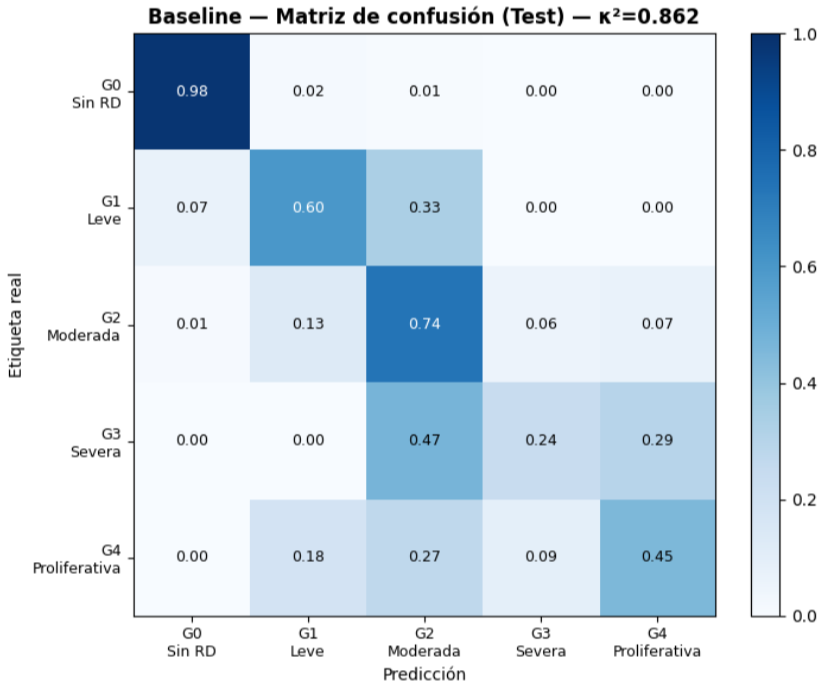
\includegraphics[width=0.8\textwidth]{baseline_conf_matrix.png}
    \caption{Matriz de confusión del Baseline}
    \label{fig:confusion_baseline}
\end{figure}

\subsection{Exp.~A --- Sobremuestreo}

$\kappa^2 = 0{,}880$ \quad F1 $= 0{,}631$

El gran beneficiario es \textbf{G2 (Moderada)}, que sube de F1 $= 0{,}715$
a $0{,}775$: al disponer de más muestras de clases minoritarias, el modelo
se atreve con predicciones que antes evitaba, dejando de refugiarse en G0
como clase segura. El kappa sube ligeramente respecto al baseline y el F1
macro mejora al ganar sensibilidad en varias clases. No obstante, G3 apenas
mejora ($0{,}276 \to 0{,}286$), lo que sugiere que la resolución de 224~px
sigue siendo insuficiente para captar las diferencias sutiles que definen
este grado.

\subsection{Exp.~D y E --- Pipelines jerárquicos}

\begin{tabular}{lcc}
\toprule
& $\kappa^2$ & F1 macro \\ \midrule
D --- Dos etapas    & 0,860 & \textbf{0,631} \\
E --- Tres niveles  & 0,855 & 0,602 \\ \bottomrule
\end{tabular}

\vspace{6pt}
Los Exp.~D y E representan un cambio de estrategia: pasar de un modelo
único a una estructura jerárquica de ``divide y vencerás''. El objetivo
no era tanto subir el kappa global como \textbf{mejorar la precisión
diagnóstica por clase}, y en eso el Exp.~D destaca: obtiene el
\textbf{mejor F1 macro del proyecto} ($0{,}631$, empatado con A) y mejora
notablemente G4 Proliferativa ($0{,}59$ frente al $0{,}51$ del
baseline), la clase clínicamente más crítica. Al separar el screening
(G0 vs resto) de la gradación (G1--G4), cada submodelo ve un problema
más equilibrado y especializado. Aunque el kappa queda ligeramente por
debajo del preentrenamiento masivo (Exp.~J), esta estructura es la
\textbf{más eficaz para distinguir clases entre sí}.

\subsection{Exp.~C --- BiomedCLIP zero-shot}

\begin{tabular}{lcc}
\toprule
\textbf{Tipo de prompt} & $\kappa^2$ & F1 macro \\ \midrule
Etiquetas simples     & 0,711 & 0,354 \\
Descripciones clínicas & 0,515 & 0,220 \\ \bottomrule
\end{tabular}

\vspace{6pt}
Las etiquetas simples funcionan mejor que las descripciones detalladas,
pero en ambos casos los valores de F1 son muy bajos. Esto nos dice que
para un problema médico de esta complejidad, el enfoque zero-shot no
puede ofrecer la precisión que requiere un ajuste fino supervisado. El
experimento confirma que \textbf{sí necesitamos entrenar un modelo
específico} ---como de hecho estamos haciendo--- y descarta la vía
del clasificador ``listo para usar'' sin entrenamiento.

\subsection{Exp.~F --- 384~px + Regresión ordinal}

$\kappa^2 = 0{,}872$ \quad F1 $= 0{,}507$

Dejamos de tratar los grados como cubos aislados y empezamos a verlos como
una \textbf{progresión continua}: una única neurona de salida, MSELoss y
umbrales optimizados con Nelder-Mead. Se sube la resolución a 384~px para
preservar detalles finos. El resultado en kappa es sólido y la matriz de
confusión muestra un \textbf{buen desempeño en G2}, sugiriendo que ahora
el modelo sí distingue microaneurismas y hemorragias que antes eran
indistinguibles. Sin embargo, el mayor problema es grave: de 33 imágenes
de G4 Proliferativa en test, \textbf{el modelo solo detecta 3}
(recall $= 9{,}1\,\%$, F1~$= 0{,}158$). La MSELoss con desbalance provoca
una compresión hacia el centro que infradiagnostica la clase más peligrosa.
Al analizar la interpretabilidad con Grad-CAM, se observa que el modelo
activa correctamente sobre estructuras clínicas en varias imágenes, pero
en otras persisten activaciones periféricas ---un comportamiento mixto
que motiva la intervención del Exp.~G.

\begin{figure}[H] % <--- Cambiado a [H] para forzar la posición exacta
    \centering
    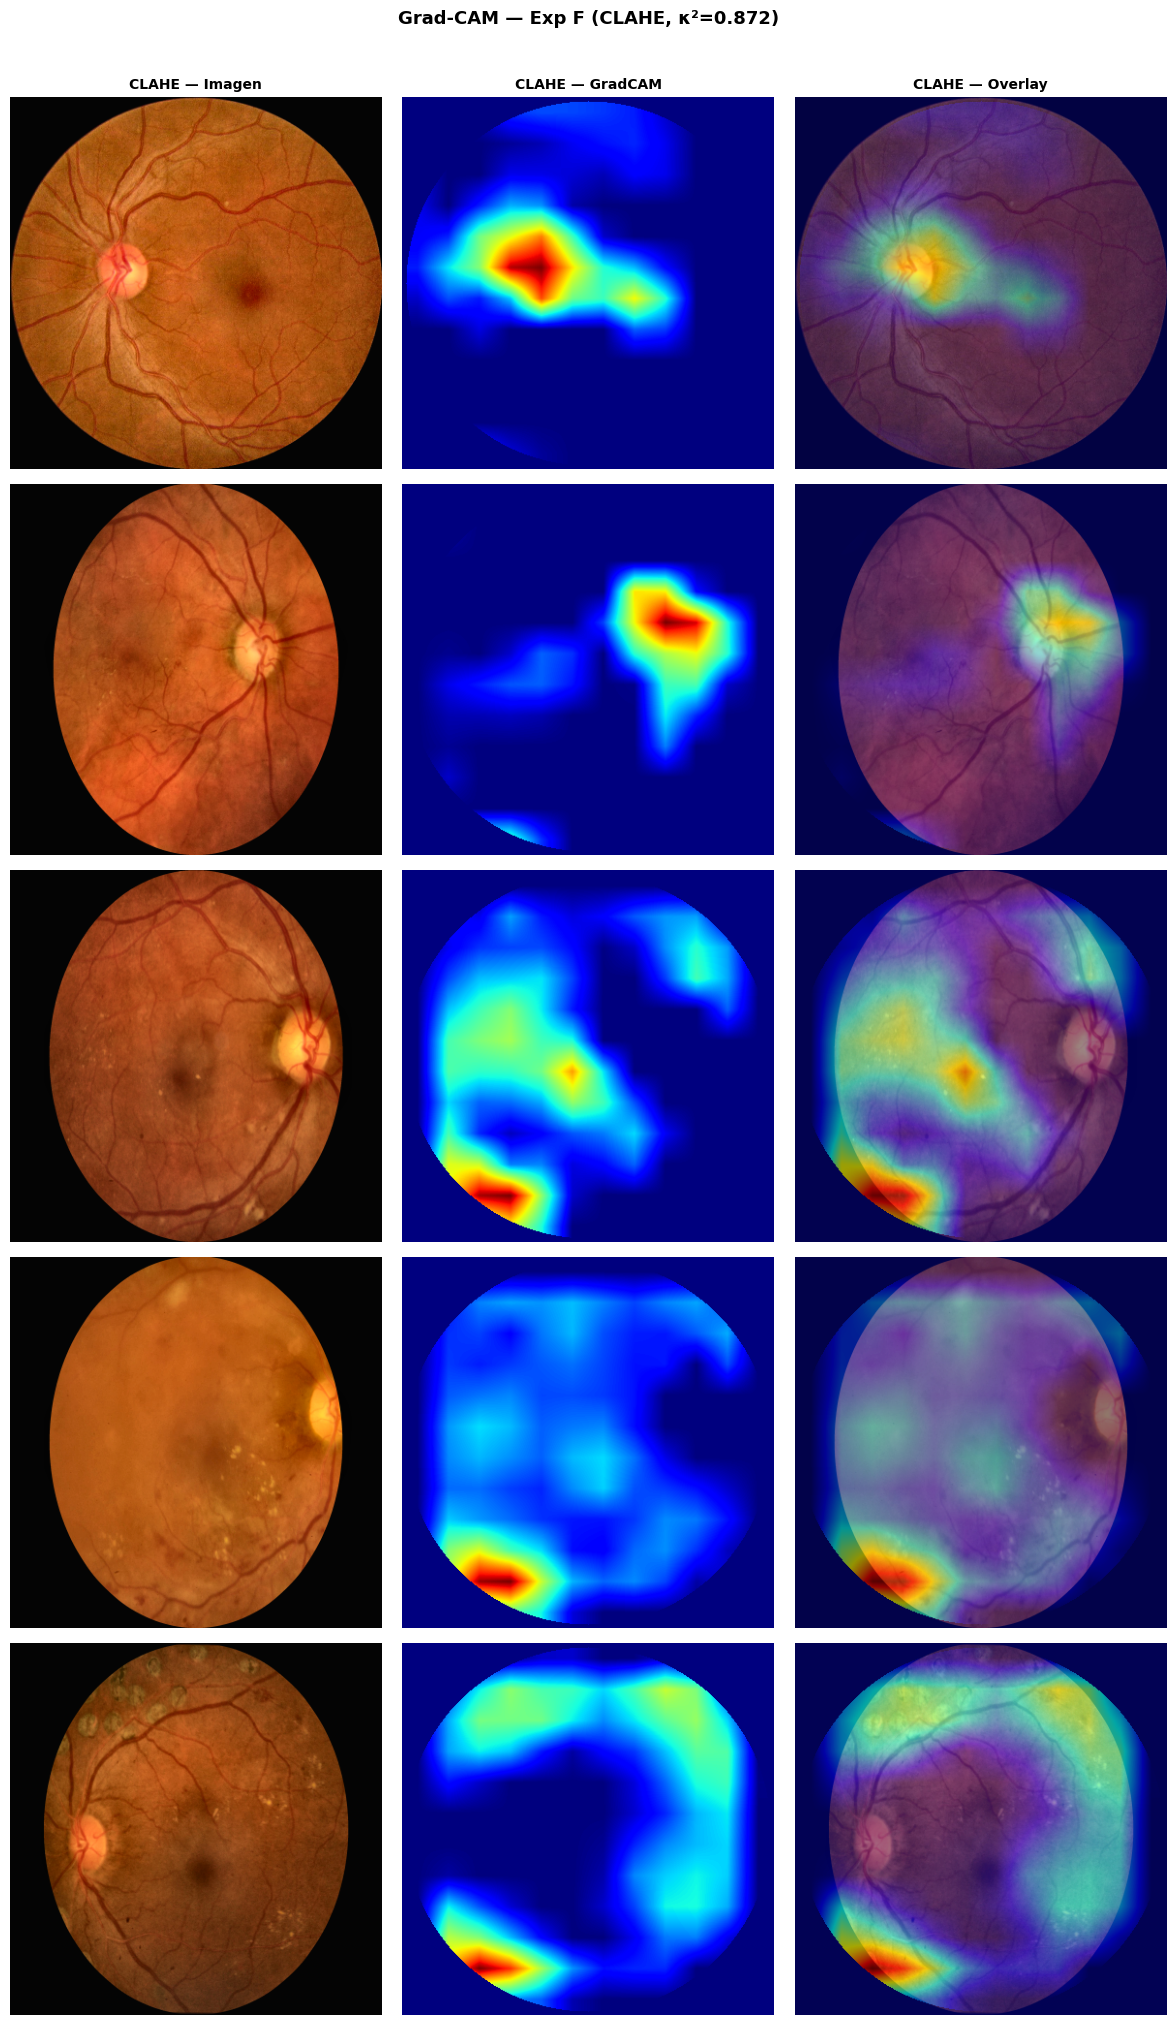
\includegraphics[width=0.5\textwidth]{grad_cam_exp_F.png}
    \caption{Visualización de Grad-CAM para el Experimento F.}
    \label{fig:grad_cam_F}
\end{figure}

\subsection{Exp.~G --- Ben Graham + máscara dura}

$\kappa^2 = 0{,}882$ \quad F1 $= 0{,}575$

Se aplica el filtro de Graham ---un filtro de paso alto que elimina la
información de baja frecuencia, dejando bordes y texturas finas--- junto
con una máscara dura a nivel de tensor y augmentaciones puramente
fotométricas. El kappa sube (+0,01 respecto a F), confirmando que la
homogeneización de la iluminación entre dispositivos mejora la
generalización. Sin embargo, la interpretabilidad con Grad-CAM empeora
respecto al Exp.~F: las activaciones se dispersan hacia la periferia del
disco en lugar de concentrarse sobre las lesiones. La explicación es que
Grad-CAM visualiza la última capa convolucional, que opera a resolución
muy baja (7$\times$7), y a esa escala lo que domina son precisamente los
bordes de alto contraste que Graham amplifica. Este resultado es el
\textbf{hallazgo más importante del proyecto}: demuestra empíricamente
que \textbf{un modelo con mejor métrica no es necesariamente un modelo
más interpretable ni más fiable}.

\subsection{Exp.~B --- Radiómica + Regresión Logística L1}

$\kappa^2 = 0{,}722$ \quad F1 $= 0{,}479$

Los resultados cuantitativos son modestos, pero el valor del experimento
no reside en ellos: reside en la \textbf{interpretabilidad}. Los
coeficientes L1 supervivientes (82 de 83 features con $C=3$) demuestran
que en las retinografías \textbf{sí existen patrones geométricos y de
contraste estadísticamente significativos} para la gradación. Por ejemplo,
para G3 los coeficientes más altos corresponden a
\texttt{firstorder\_10Percentile} (negativo: las hemorragias bajan la
intensidad mínima) y \texttt{glrlm\_HighGrayLevelRunEmphasis} (positivo:
los exudados producen rachas brillantes). Este diccionario
feature$\to$significado clínico es imposible de extraer del CNN.

\subsection{Exp.~I --- Fusión CNN + Radiómica}

$\kappa^2 = 0{,}855$ (LightGBM) \quad F1 $= 0{,}631$ (LightGBM)

Al fusionar 1\,536 deep features del Exp.~G con las 107 radiómicas, los
resultados revelan información clara sobre \textbf{qué es realmente
valioso para diagnosticar RD}: el 96,5\,\% de la aportación relativa
proviene de la CNN. Sin embargo, al mirar el F1 macro ($0{,}631$)
comprobamos que mejora sustancialmente respecto al Exp.~B ($0{,}479$) y
al Exp.~C ($0{,}354$). La inclusión de características radiómicas ayuda
al modelo a ser \textbf{más preciso en las clases difíciles} (G1, G3)
donde antes dudaba más.

\subsection{Exp.~J --- Preentrenamiento con APTOS 2015}

$\kappa^2 = \mathbf{0{,}885}$ \quad F1 $= 0{,}551$

\textbf{Mejor kappa del proyecto.} La estrategia es directa: preentrenar
20 épocas en las 35\,k imágenes de APTOS~2015 y fine-tunear en 2019 con
LR reducida ($2{\times}10^{-5}$). Lo revelador es que desde la primera
época de fine-tuning el modelo ya alcanza $\kappa^2 = 0{,}883$: no está
intentando entender qué es una retina ---eso ya lo aprendió con las 35\,k
imágenes--- sino que está \textbf{ajustando los detalles específicos} del
dataset de 2019. Además, mejora la detección de G4 Proliferativa con un
recall del 27,3\,\%: puede parecer bajo en términos absolutos, pero es un
progreso enorme respecto al 9,1\,\% del Exp.~F. Este modelo es mucho más
\textbf{resiliente} frente a la variabilidad de las imágenes, precisamente
porque ha visto una diversidad real de dispositivos y centros durante el
preentrenamiento.

\subsection{Comparativa final}

\begin{table}[H]
\centering
\small
\caption{Comparativa global ordenada por $\kappa^2$ en test.}
\label{tab:comparativa}
\begin{tabularx}{\textwidth}{l X c c}
\toprule
\rowcolor{azuloscuro!15}
\textbf{Exp.} & \textbf{Técnica} & $\boldsymbol{\kappa^2}$ & \textbf{F1} \\
\midrule
\textbf{J} & Pretrain APTOS 2015 $\to$ Fine-tune 2019
           & \textbf{0,885} & 0,551 \\
\rowcolor{grisclaro}
G & Ben Graham + máscara dura + aug.\ fotométricas
  & 0,882 & 0,575 \\
A & Sobremuestreo clases minoritarias
  & 0,880 & 0,631 \\
\rowcolor{grisclaro}
F & 384~px + MSELoss + umbrales Nelder-Mead
  & 0,872 & 0,507 \\
Baseline & EfficientNet-B3 + Weighted CE (224~px)
         & 0,862 & 0,602 \\
\rowcolor{grisclaro}
D & Binario RD$+$/RD$-$ + Severidad G1--G4
  & 0,860 & \textbf{0,631} \\
E & Jerárquico 3 niveles
  & 0,855 & 0,602 \\
\rowcolor{grisclaro}
I & Deep feats + Radiómica $\to$ LightGBM
  & 0,855 & 0,631 \\
B & PyRadiomics + LR L1
  & 0,722 & 0,479 \\
\rowcolor{grisclaro}
C & BiomedCLIP zero-shot (prompts genéricos)
  & 0,711 & 0,354 \\
\bottomrule
\end{tabularx}
\end{table}

\begin{figure}[H] 
    \centering
    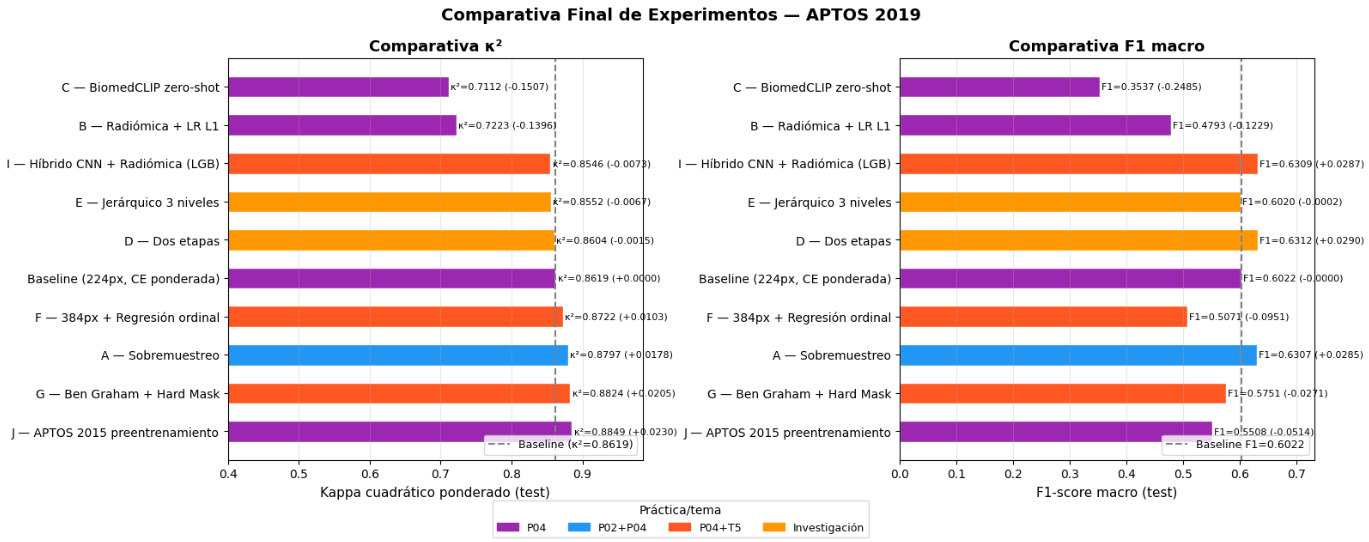
\includegraphics[width=1\textwidth]{comparativa_final.png}
    \caption{Comparativa Final de Experimentos.}
    \label{fig:comparativa_final}
\end{figure}

\newpage

\section{Conclusiones y vías futuras}
\label{sec:conclusiones}
\subsection{Conclusiones}

El proyecto ha construido un pipeline completo de gradación automática de
retinopatía diabética, partiendo de un baseline sólido ($\kappa^2 = 0{,}862$)
y explorando diez experimentos que atacan sus limitaciones de forma iterativa.
Las principales lecciones son:

\begin{enumerate}
  \item \textbf{El desbalance necesita variedad, no volumen.} Replicar datos
        (Exp.~A) apenas mejora G3; incorporar 35\,k imágenes reales
        (Exp.~J) sí funciona ($\kappa^2 = 0{,}885$).
  \item \textbf{Dividir el problema ayuda.} El pipeline jerárquico (Exp.~D)
        logra el mejor F1 macro y la mayor mejora en G4, la clase más
        crítica.
  \item \textbf{Métrica alta $\neq$ modelo fiable.} El Exp.~G sube
        $\kappa^2$ pero empeora Grad-CAM respecto a F: la auditoría de
        interpretabilidad es tan necesaria como la evaluación cuantitativa.
  \item \textbf{El entrenamiento específico es imprescindible.} Radiómica
        (B) y zero-shot (C) quedan 14--15 puntos por debajo del CNN,
        pero B aporta interpretabilidad que el CNN no puede ofrecer.
\end{enumerate}

\subsection{Limitaciones}
\begin{itemize}
  \item \textbf{Tiempo y cómputo.} No se pudo ejecutar el baseline a
        384~px ni probar más épocas, lo que habría aislado mejor el
        efecto de la resolución frente al de la regresión ordinal.
  \item \textbf{Interpretabilidad solo cualitativa.} Grad-CAM se evalúa
        por inspección visual; falta una métrica objetiva sobre lesiones
        anotadas.
  \item \textbf{Sin validación externa.} Todos los resultados provienen
        de APTOS~2019; la generalización a otros centros y equipos queda
        sin cuantificar.
\end{itemize}

\subsection{Vías futuras}
\begin{itemize}
  \item Fine-tuning diferencial (congelar capas iniciales) y backbones
        más recientes (ConvNeXt, EfficientNetV2).
  \item Resolución de 448--512~px para preservar microlesiones de G1.
  \item Interpretabilidad cuantitativa mediante \textit{pointing game}
        sobre anotaciones de lesiones (IDRiD).
\end{itemize}

% ══════════════════════════════════════════════════════════════════════════════
%  BIBLIOGRAFÍA
% ══════════════════════════════════════════════════════════════════════════════
\newpage
\printbibliography[heading=bibintoc, title={Bibliografía}]

% ══════════════════════════════════════════════════════════════════════════════
%  ANEXO
% ══════════════════════════════════════════════════════════════════════════════
\newpage
\appendix
\section{Tabla de contribución individual}
\label{sec:contribucion}

\begin{table}[H]
  \centering
  \caption{Distribución de tareas entre los miembros del grupo. \\
    \textbf{R}\,=\,responsable principal, \textbf{P}\,=\,participó.}
  \label{tab:contribucion}
  \begin{tabularx}{\textwidth}{X c c c}
    \toprule
    \rowcolor{azuloscuro!15}
    \textbf{Tarea} &
    \textbf{\small Javier G.} &
    \textbf{\small Miguel Á. V.} &
    \textbf{\small Martín S.} \\
    \midrule
    Exploración del dataset (EDA)           & R & P & P \\
    \rowcolor{grisclaro}
    Preprocesamiento (máscara, CLAHE)       & R & P & P \\
    Dataset class y aumentación             & R & P & P \\
    \rowcolor{grisclaro}
    Baseline (EfficientNetBN-B3)            & R & P & P \\
    Exp. A --- Sobremuestreo                & P & R & P \\
    \rowcolor{grisclaro}
    Exp. B --- Radiómica + LR L1            & P & P & R\\
    Exp. C --- BiomedCLIP zero-shot         & P & P & R \\
    \rowcolor{grisclaro}
    Exp. D --- Pipeline dos etapas          & P & R & P \\
    Exp. E --- Jerárquico tres niveles      & P & R & P \\
    \rowcolor{grisclaro}
    Exp. F --- 384\,px + Regresión ordinal  & P & R & P \\
    Exp. G --- Ben Graham + Hard Mask       & P & P & R \\
    \rowcolor{grisclaro}
    Interpretabilidad Grad-CAM             & P & P & P \\
    Exp. I --- Híbrido CNN + Radiómica      & P & P & R\\
    \rowcolor{grisclaro}
    Exp. J --- Pretrain APTOS 2015          & P & P & R \\
    Redacción de la memoria                 & P & P & P \\
    \rowcolor{grisclaro}
    Preparación de la defensa               & P & P & P \\
    \bottomrule
  \end{tabularx}
\end{table}

\end{document}
